\chapter{The Big Picture}
\section{Introduction}
SQLMap is a simple but complete framework that makes it easy for you to map
your objects to your SQL statements or stored procedures. The goal of the
SQLMap framework is to obtain 80\% of data access functionality using only
20\% of the code.

\section{What does it do?}
Developers often create maps between objects within an application. One
definition of a Mapper is an ``object that sets up communication between two
independent objects.'' A Data Mapper is a ``layer of mappers that moves data
between objects and a database while keeping them independent of each other
and the mapper itself.'' [Patterns of Enterprise Architecture, ISBN
0-321-12742-0].

You provide the database and the objects; SQLMap provides the mapping layer
that goes between the two.

\section{How does it work?}

Your programming platform already provides a capable library for accessing
databases, whether through SQL statements or stored procedures. But developers
find several things are still hard to do well when using ``stock'' PHP
function including:

Separating SQL code from programming code Passing input parameters to the
library classes and extracting the output Separating data access classes from
business logic classes Caching often-used data until it changes Managing
transactions and many more -- by using XML documents to create a mapping
between a plain-old object and a SQL statement or a stored procedure. The
``plain-old object'' can be any PHP object.

\begin{mybox}{Tip:}
The object does not need to be part of a special object hierarchy or implement
a special interface. (Which is why we call them ``plain-old'' objects.)
Whatever you are already using should work just fine.
\end{mybox}

\begin{figure}[!h]
    \centering
        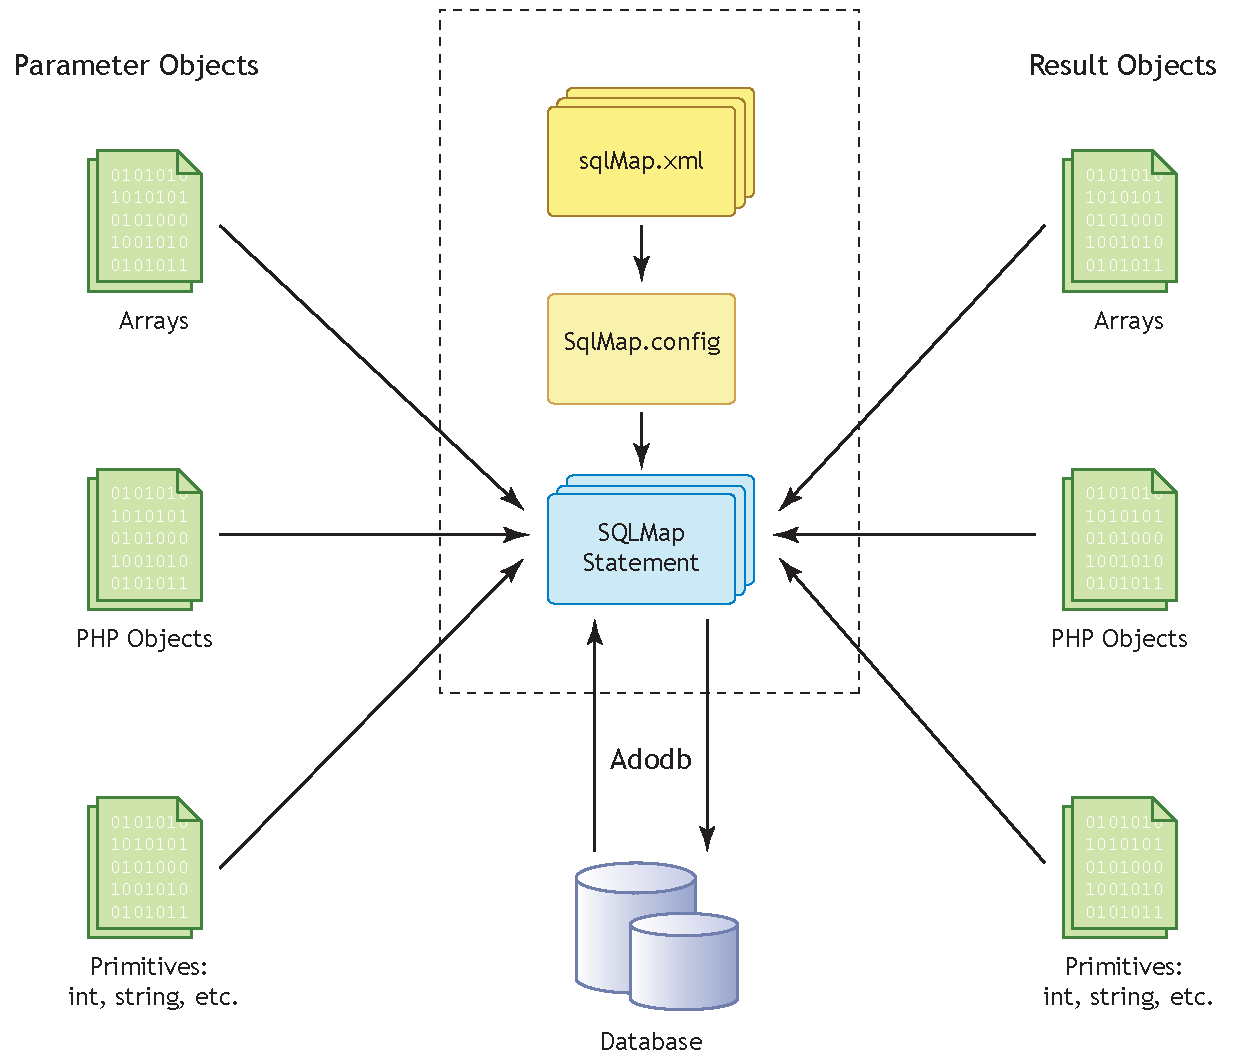
\includegraphics[width=0.65\textwidth]{diagram}
    \caption{SQLMap DataMapper work flow}
    \label{fig:diagram}
\end{figure}

Here's a high level description of the work flow diagrammed by
Figure~\ref{fig:diagram}: Provide a parameter, either as an object or a
primitive type. The parameter can be used to set runtime values in your SQL
statement or stored procedure. If a runtime value is not needed, the parameter
can be omitted.

Execute the mapping by passing the parameter and the name you gave the
statement or procedure in your XML descriptor. This step is where the magic
happens. The framework will prepare the SQL statement or stored procedure, set
any runtime values using your parameter, execute the procedure or statement,
and return the result.

In the case of an update, the number of rows affected is returned. In the case
of a query, a single object, or a collection of objects is returned. Like the
parameter, the result object, or collection of objects, can be a plain-old
object or a primitive type.

So, what does all this look like in your source code? Here's how you might
code the insert of a ``lineItem'' object into your database.

\begin{verbatim}
TMapper::instance()->insert("InsertLineItem", $lineItem);
\end{verbatim}

If your database is generating the primary keys, the generated key can be
returned from the same method call, like this:

\begin{verbatim}
$myKey = TMapper::instance()->insert("InsertLineItem", $lineItem);
\end{verbatim}

Example~\ref{example:2.1} shows an XML descriptor for ``InsertLineItem''.
\begin{example}\label{example:2.1}
The ``InsertLineItem'' descriptor
\begin{verbatim}
<insert id="InsertLineItem" parameterClass="LineItem">
  INSERT INTO [LinesItem]
    (Order_Id, LineItem_LineNum, Item_Id, LineItem_Quantity, LineItem_UnitPrice)
  VALUES
    (#Order.Id#, #LineNumber#, #Item.Id#, #Quantity#, #Item.ListPrice#)
 <selectKey type="post" resultClass="int" property="Id" >
  select @@IDENTITY as value
 </selectKey>
</insert>
\end{verbatim}
\end{example}

The \tt{<selectKey>} stanza returns an auto-generated key from a SQL Server
database (for example). If you need to select multiple rows, SQLMap can return
a list of objects, each mapped to a row in the result set:
\begin{verbatim}
$productList = Mapper::instance()->queryForList("selectProduct",$categoryKey);
\end{verbatim}
Or just one, if that's all you need:
\begin{verbatim}
$product = Mapper::instance()->queryForObject("selectProduct",$categoryKey);
\end{verbatim}

Of course, there's more, but this is SQLMap from 10,000 meters. (For a longer,
gentler introduction, see the Tutorial.) Section~\ref{section:3} describes the
Data Map definition files -- where the statement for ``InsertLineItem'' would
be defined. The Developers Guide for PHP (Section~\ref{section:4}) describes
the "bootstrap" configuration file that exposes SQLMap to your application.

\section{Is SQLMap the best choice for my project?}
SQLMap is a Data Mapping tool. Its role is to map the columns of a database
query (including a stored procedure) to the properties of an object. If your
application is based on business objects (including array or lists of
objects), then SQLMap can be a good choice. SQLMap is an even better choice
when your application is layered, so that that the business layer is distinct
from the user-interface layer.

Under these circumstances, another good choice would be an Object/Relational
Mapping tool (OR/M tool), like [...]. Other products in this category are
[...] and [...] . An OR/M tool generates all or most of the SQL for you,
either beforehand or at runtime. These products are called OR/M tools because
they try to map an object graph to a relational schema.

SQLMap is not an OR/M tool. SQLMap helps you map objects to stored procedures
or SQL statements. The underlying schema is irrelevant. An OR/M tool is great
if you can map your objects to tables. But they are not so great if your
objects are stored as a relational view rather than as a table. If you can
write a statement or procedure that exposes the columns for your object,
regardless of how they are stored, SQLMap can do the rest.

So, how do you decide whether to OR/M or to DataMap? As always, the best
advice is to implement a representative part of your project using either
approach, and then decide. But, in general, OR/M is a good thing when you
\begin{itemize}
  \item Have complete control over your database implementation.
  \item Do not have a Database Administrator or SQL guru on the team.
  \item Need to model the problem domain outside the database as an object graph.
\end{itemize}
Likewise, the best time to use a Data Mapper, like SQLMap, is when:
\begin{itemize}
  \item You do not have complete control over the database implementation, or want to
continue to access a legacy database as it is being refactored.
  \item You have database administrators or SQL gurus on the team.
  \item The database is being used to model the problem domain, and the application's
primary role is to help the client use the database model.
\end{itemize}

In the end, you have to decide what's best for your project. If a OR/M tool
works better for you, that's great! If your next project has different needs,
then we hope you give SQLMap another look. If SQLMap works for you now:
Excellent!
